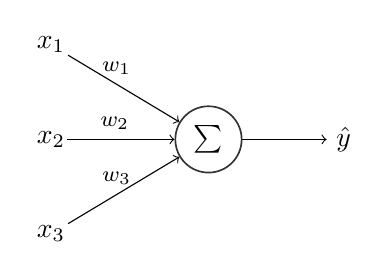
\begin{tikzpicture}
	\tikzstyle{neuron} = [circle,draw=black!80,semithick,minimum size=20pt]
	% input layer
	\foreach \i in {1,...,3}
		\node (input\i) at (0, -\i*1.2) {$x_\i$};
	% perceptron
	\node[neuron] (perceptron) at (2, -2*1.2) {$\sum$};
	% connections
	\foreach \i in {1,...,3}
		\draw[->, shorten <= -.1cm] (input\i) -- node[pos=.4,above]{\footnotesize{$w_\i$}} (perceptron);
	% output
	\draw[->] (perceptron) -- node[above]{$\sign$}(3.5, -2*1.2) node[right]{$\hat{y}$};
\end{tikzpicture}